%% Placeholder for chapter on convexity

%Below are notes for Oct23
\section{Linear/affine/convex/conic hulls \& sets}
Given a set of points $x^{(i)} \in \Re^n$, $i\in [m]$

\begin{equation*}
P = \{x^{(1)}, x^{(2)},..., x^{(m)} \}
\end{equation*}

Consider combinations of form $\sum^m_{i=1} \lambda_i x^{(1)}$

1) The "linear" hull: 

\begin{equation*}
\{x|x = \sum^m_{i=1} \lambda_i x^{(i)}, \lambda_r\in \Re, \forall i\in [m] \}
\end{equation*}

2) The "affine" hull: 

\begin{equation*}
\{x|x = \sum^m_{i=1} \lambda_i x^{(i)}, \lambda_i\in \Re, \sum^n_{i=1}\lambda_i = 1 \}
\end{equation*}


3) The "convex" hull: 

\begin{equation*}
\{x|x = \sum^m_{i=1} \lambda_i x^{(i)}, \lambda_i\in \Re, \lambda_i \geq 0, \sum^m_{i=1}\lambda_i = 1 \}
\end{equation*}


4) The "conic" hull: 

\begin{equation*}
\{x|x = \sum^m_{i=1} \lambda_i x^{(i)}, \lambda_i\in \Re, \lambda_i \geq 0 \}
\end{equation*}


\begin{center}
	\begin{tabular}{|c|c|c|}
	\hline  
   & $\lambda_i \geq 0$   & $\sum^m_{i=1}\lambda_i = 1$ \\
	\hline  
Linear&  no  & no \\
	\hline  
Affine&  no  &yes  \\
	\hline 
Covex&  yes  & yes \\
	\hline  
Conic&  yes  &  no\\
	\hline 
\end{tabular}
\end{center}



1) Linear Hull

Linear hull of $P = span\{x^{(1)},...,x^{(m)} \} =span(P)$

$\rightarrow$ smallest subspace that contains $P$.

2) Affine hull

\begin{align*}
P &= \{x^{(1)}, x^{(2)} \}\\
x &= \lambda_1x^{(1)} + \lambda_2x^{(2)}\\
&= \lambda_1x^{(1)} + (1-\lambda)_1x^{(1)}\\
&= x^{(2)} + \lambda(x^{(1)} - x^{(2)})\\
aff(P) &= x^{(2)} + span(x^{(1)} - x^{(2)})
\end{align*}

\begin{align*}
P &= \{x^{(1)}, x^{(2)}, x^{(3)} \}\\
x &= \lambda_1x^{(1)} + \lambda_2x^{(2)} + \lambda_3x^{(3)}\\
&= (1 - \lambda_2 - \lambda_3)x^{(1)} + \lambda_2x^{(2)} + \lambda_3x^{(3)}\\
&= x^{(1)} + \lambda_2(x^{(2)} - x^{(1)}) + \lambda_3(x^{(3)} - x^{(1)})
\end{align*}

\begin{marginfigure}
	\centering
	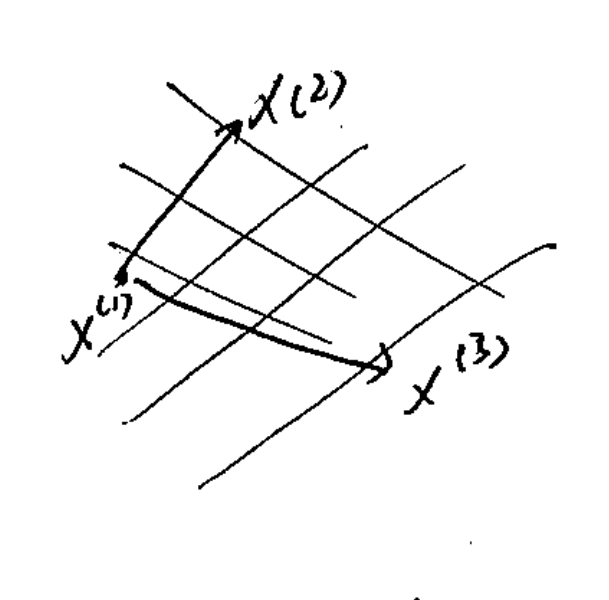
\includegraphics[width=1.8in,height=1.8in]{figures/ch08/figure1023_1.png}
	%\caption{This is an inserted JPG graphic} 
	%\label{fig:graph} 
\end{marginfigure}

3) Convex hulls

\begin{align*}
P &= \{x^{(1)},  x^{(2)}\}\\
x &= \lambda_1x^{(1)} + \lambda_2x^{(2)}\\
&= (1-\lambda)x^{(1)} + \lambda x^{(2)}\\
&= x^{(1)} + \lambda(x^{(2)} - x^{(1)})
\end{align*}

\begin{align*}
P &= \{x^{(1)},  x^{(2)}, x^{(3)} \}\\
x &= \lambda_1x^{(1)} + \lambda_2x^{(2)} + \lambda_3x^{(3)}\\
&= x^{(1)} + \lambda_2(x^{(2)} - x^{(1)}) + \lambda_3(x^{(3)} - x^{(1)})\\
&= x^{(1)} + \lambda \gamma(x^{(2)} - x^{(1)}) + (1 - \lambda)\gamma(x^{(3)} - x^{(1)})
\end{align*}


\begin{marginfigure}
	\centering
	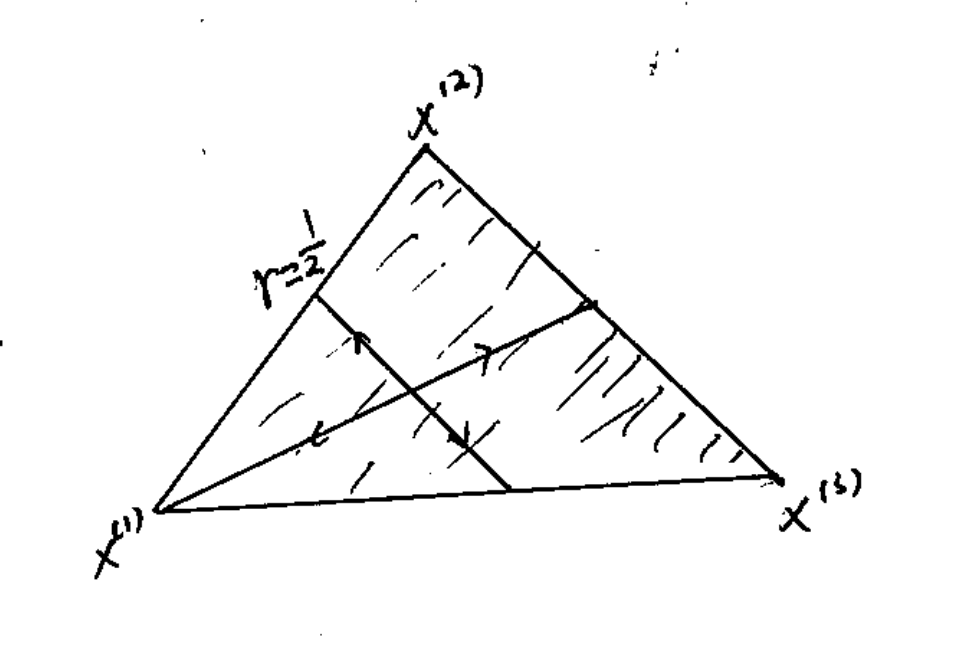
\includegraphics[width=1.8in,height=1.8in]{figures/ch08/figure1023_2.png}
	%\caption{This is an inserted JPG graphic} 
	%\label{fig:graph} 
\end{marginfigure}

\begin{marginfigure}
	\centering
	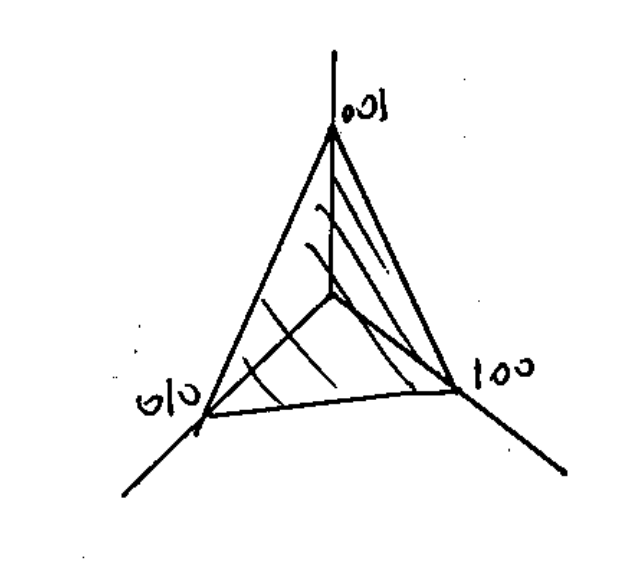
\includegraphics[width=1.8in,height=1.8in]{figures/ch08/figure1023_3.png}
	%\caption{This is an inserted JPG graphic} 
	%\label{fig:graph} 
\end{marginfigure}

4) Conic hulls: $\sum^n_{i=1}\lambda_i x^{(i)}$, $\lambda_i \geq 0$, $\forall i\in [m]$

\begin{align*}
P &= \{x^{(1)}, x^{(2)} \}\\
x &= \lambda_1x^{(1)} + \lambda_2x^{(2)}\\
&= ( \lambda_1 + \lambda_2)[\frac{\lambda_1}{\lambda_1 + \lambda_2}x^{(1)} + \frac{\lambda_2}{\lambda_1 + \lambda_2}x^{(2)}]\\
&= \gamma[\lambda x^{(1)} + (1-\lambda)x^{(2)}]
\end{align*}

\begin{marginfigure}
	\centering
	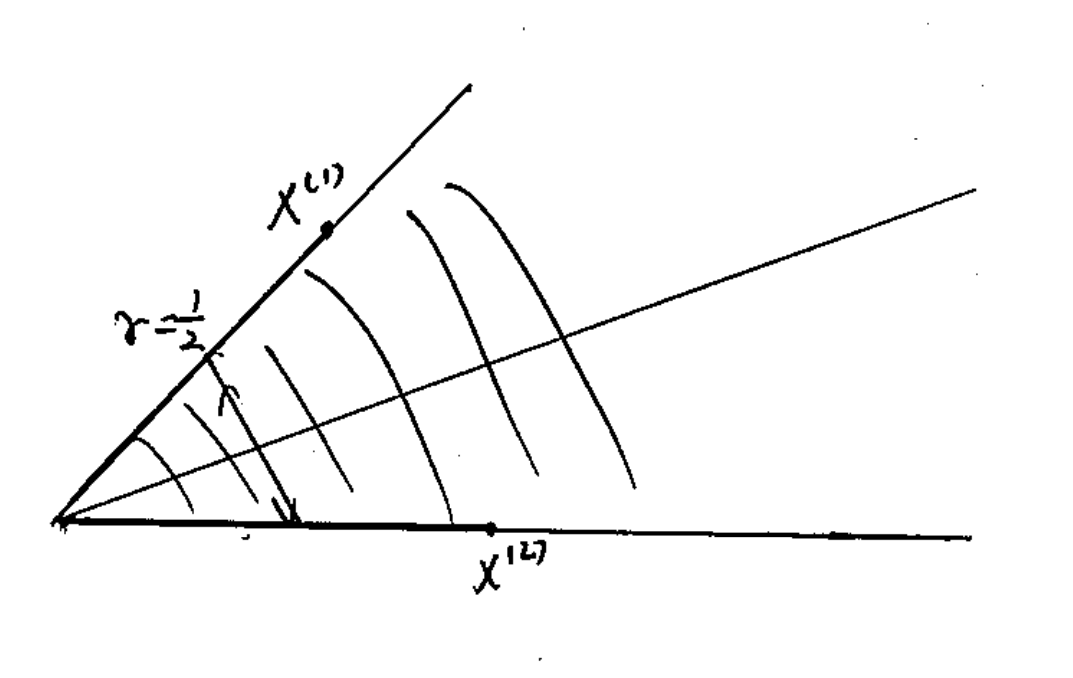
\includegraphics[width=1.8in,height=1.8in]{figures/ch08/figure1023_4.png}
	%\caption{This is an inserted JPG graphic} 
	%\label{fig:graph} 
\end{marginfigure}

\subsection{Convex Sets}

\begin{definition}{Convex}
	A subset $C\subseteq \Re^n$ is a "convex" set if $\forall x,y \in \mathcal{C}$, then $z\in \mathcal{C}$, $\forall z = \lambda x + (1-\lambda)y$, $\lambda \in [0,1]$
\end{definition}


\begin{definition}{Strictly Convex}
	A convex set is "strictly" convex if $\forall x,y \in \mathcal{C}$, $\forall \lambda \in (0,1)$, $z = \lambda x + (1-\lambda)y \in rel\,int(\mathcal{C})$(relative interior)
\end{definition}

Objects with straight edges are not strictly convex sets.

\begin{definition}{Cone}
	A set $\mathcal{C}\subseteq \Re^n $ is a cone if $\forall x\in \mathcal{C}$, then $\gamma x\in \mathcal{C}, \forall \gamma \geq 0$
\end{definition}

\begin{example}
	1) Hyper-planes are convex: $H = \{x| a^Tx = b \}$, pick $x,y \in H$, is $z =\lambda x + (1-\lambda)y \in H$? $\forall \lambda \in [0,1]$
	
	\begin{align*}
	a^Tz &= a^T(\lambda x + (1-\lambda)y)\\
	&= \lambda(a^Tx) + (1-\lambda)y\\
	&= \lambda b + (1-\lambda)b\\
	&= b
	\end{align*}
	
	
	2) Half-space: $\{x|a^Tx = b \}$, same proof except get inequality here in above equations($a^Tz \neq \lambda b + (1-\lambda)b$).
	
	3) If $c_1, ..., c_n$ al convex sets, then $\mathcal{C} = \cap^m_{i=1}$ is convex.
	
	\begin{proof}
		Pick any $x,y\in \mathcal{C}$ $\Rightarrow$ $x,y\in \mathcal{C}_i,\forall i\in [m]$.
		
		Consider any $z = \lambda x + (1 - \lambda)y$ , is this in $\mathcal{C}$?
		
		Since $x,y \in \mathcal{C}$, $\rightarrow z\in \mathcal{C}_i$ since $\mathcal{C}_i$, $\forall i\in [m]$
		
		If $z\in \mathcal{C}_i$, $\forall i\in [m]$ also intersection $\rightarrow z\in \cap^m_{i=1}C_i = C$
		
	\end{proof}

	In LP $\&$ QP Feasible set:
	
	\begin{equation*}
	\{x|Ax = b \}\cap \{x|Gx\leq b \} = \{\cap^q_{i=1}\{x|a^{(i)^T}x = b_i  \}\cap \{\cap^m_{i=1}\{x|g^{(i)^T}x \leq h_i \}
	\end{equation*}
	
	4) Affine transformations:
	
	If a map $F: \Re^n \rightarrow \Re^m$ is affine ($F(x) = Ax + b$) and $\mathcal{C} \subseteq \Re^n$ is convex, then the image of $\mathcal{C}$ under $F$ is convex.
	
	\begin{equation*}
	F(\mathcal{C}) = \{F(x) | x\in \mathcal{C} \} \subseteq \Re^m
	\end{equation*}

	Also pre-image of a convex set $\tilde{e}$ in $\Re^m$ is convex
	
	\begin{equation*}
	\{x|F(x)\in \mathcal{C} \} \subseteq \Re^n
	\end{equation*}
\end{example}

\begin{marginfigure}
	\centering
	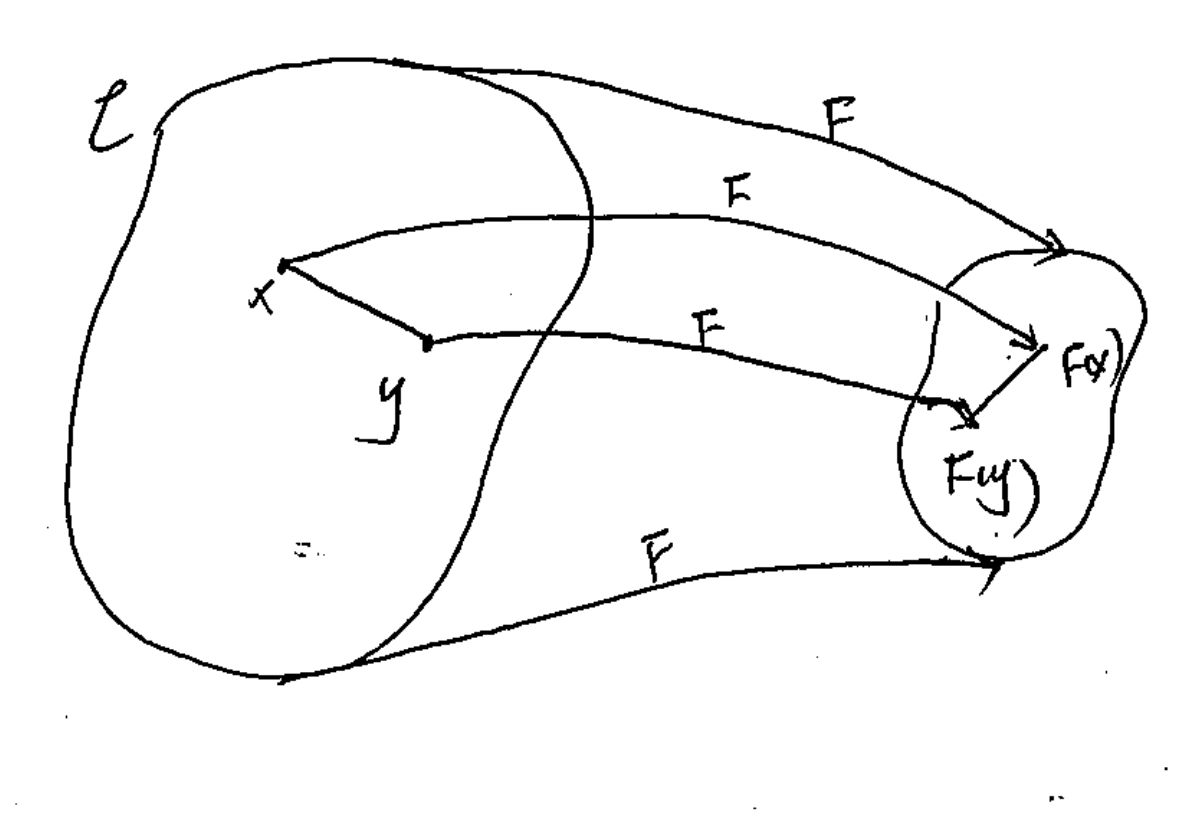
\includegraphics[width=1.8in,height=1.8in]{figures/ch08/figure1023_5.png}
	%\caption{This is an inserted JPG graphic} 
	%\label{fig:graph} 
\end{marginfigure}


Norm balls are convex

\begin{marginfigure}
	\centering
	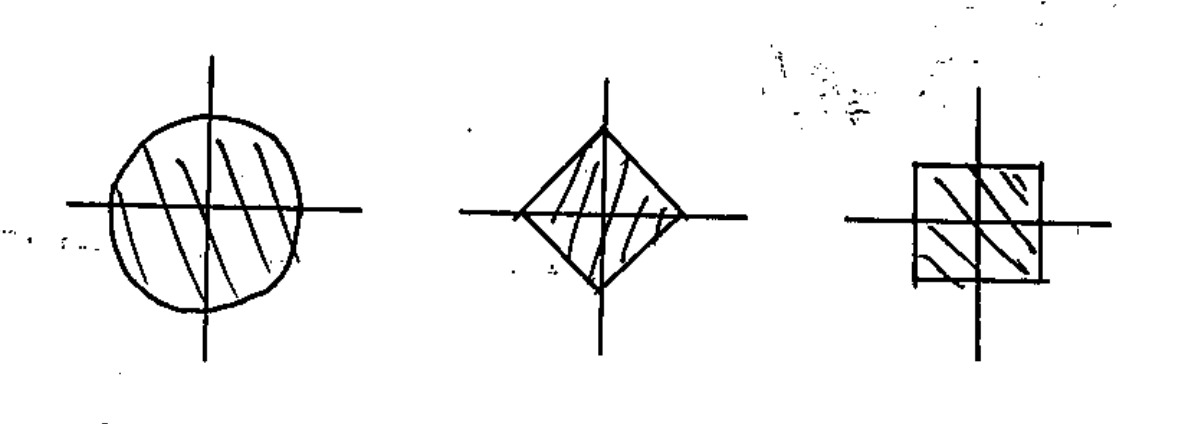
\includegraphics[width=1.8in,height=1.8in]{figures/ch08/figure1023_6.png}
	%\caption{This is an inserted JPG graphic} 
	%\label{fig:graph} 
\end{marginfigure}

\begin{proof}
	Take any two points $u,v$ s.t. $\Vert u\Vert \leq 1$, $\Vert v\Vert \leq 1$. 
	
	\begin{align*}
	\Vert \lambda u+(1-\lambda)v\Vert &\leq \Vert \lambda u\Vert + \Vert (1-\lambda)v\Vert\\
	&= \vert \lambda \vert \Vert  u\Vert + \vert (1-\lambda) \vert \Vert  v\Vert\\
	&= \lambda\Vert  u\Vert + (1-\lambda)\Vert  v\Vert\\
	&\leq \lambda 1 + (1-\lambda)1\\
	&= 1
	\end{align*}
	
	\begin{equation*}
	\Vert  x\Vert_p = (\sum^n_{i=1}\vert  x_i\vert^p)^{\frac{1}{p}}
	\end{equation*}
	norm if $p\geq 1$
\end{proof}

\subsection{Ellipsoids}

\begin{equation*}
\xi(x_c, P) =\{x|(x - x_c)^TP^{-1}(x - x_c) \leq 1 \}
\end{equation*}
where $P\in S^n_{++}$   is a convex set.

\begin{proof}
	
	$l_2$ norm ball is convex. 
	
	Consider following affine map $F(u) = P^{\frac{1}{2}}u + x_c$.
	
	The set $\{F(u) | \Vert y\Vert_2 \leq 1 \}$ is convex. 
\end{proof}

Define a set:

\begin{align*}
\{F(u) | \Vert u\Vert^2_2 \leq 1 \} &= \{x|x = P^{\frac{1}{2}}u+x_c, \Vert u\Vert^2 \leq 1 \}\\
&= \{x|x - x_c = P^{\frac{1}{2}}u, \Vert u\Vert^2 \leq 1 \}\\
&= \{x|P^{-\frac{1}{2}}(x - x_c) =u, \Vert u\Vert^2 \leq 1 \}\\
&= \{x|\Vert P^{-\frac{1}{2}}(x - x_c)\Vert^2_2 \leq 1 \}\\
&= \{x|(x - x_c)^TP^{-1}(x - x_c) \leq 1 \}
\end{align*}

Intersect these shapes with polyhedron to get feasible set of QCQP.

\begin{example}
	\begin{align*}
	\{x | \Vert Ax - b \Vert^2_2 \leq 1 \} &= \{x | \Vert F(x) \Vert^2 \leq 1 \}  where F(x) = Ax - b
	\end{align*}
	
	Pre-image of convex set under an affine function and so it's convex
\end{example}


%Above are notes for Oct23


%Below are notes for Oct30
Consider an affine function $F(x) = Ax + b$, $A\in \Re^{m\times n}$, $b\in \Re^m$, $F:\Re^n \rightarrow \Re^m$

Then:

\begin{enumerate}
	\item $\forall \mathcal{C}\subseteq \Re^n$ that are convex, the image of $\mathcal{C}$ under action of $F$ is a convex set in $\Re^m$:
	
	\begin{equation*}
	F(\mathcal{C}) = \{F(x)\in \Re^m \vert x\in \mathcal{C} \}
	\end{equation*}
	
	\item $\forall \mathcal{C}\subseteq \Re^m$ that are convex, the pre-image ("inverse image") of $\mathcal{C}$ under $F$: 
	\begin{equation*}
	F^{-1}(\mathcal{C}) = \{x| F(x)\in \mathcal{C} \}
	\end{equation*}
	is a convex set $\in \Re^n$
\end{enumerate}

Used (1) show:
\begin{itemize}
	\item all norm balls are convex sets.
	
	\item ellipsoids are convex sets.
\end{itemize}

\begin{example}
	$\{x|\Vert Ax + b\Vert \leq 1 \}$ is a convex set$\rightarrow$ 
	
	Let $F(x) = Ax + b$(affine function)
	
	Let $\beta = \{x|\Vert x \Vert \leq 1 \}\in \Re^m$
	
	\begin{align*}
	\{x|\Vert Ax+b\Vert\leq 1 \} &= \{x|\Vert F(x) \Vert\leq 1 \}\\
	&= \{x|F(x) \leq \beta \}\\
	&= F^{-1}(\beta)
	\end{align*}
\end{example}


Recall:

$\mathcal{C}$ is a cone if $\forall x\in \mathcal{C}$ and $\theta \in \Re_{+}$(i,e. $\theta \geq 0$)   

Important cones: PSD matrices   


\begin{align*}
S^n &= \{x\in \Re^{n\times n}s.t. x = x^T \}\\
S^n_+ &= \{x\in S^{n}s.t. v^TXv \geq 0, \forall v\in \Re^n \}\\
S^n &= \{x\in S^{n}s.t. v^TXv > 0 ,\forall v\in \Re^n\}
\end{align*}

1) $S_+^n$ is a cone since $\forall x \in S_+^n$ and $\forall \theta \geq 0$:

\begin{equation*}
v^T(\theta X)v = \theta v^TXv  > 0
\end{equation*}

write:
\begin{align*}
X\in S^n_+ &\Leftrightarrow X\geq 0\\
X\in S^n_{++} &\Leftrightarrow X> 0
\end{align*}

2) $S_+^n$ is a convex cone.

Let $A\in S^n_+$, $B\in S^n_+$ consider $\lambda A + (1-\lambda)B$ where $\lambda \in [0,1]$

$\rightarrow$ First note $(\lambda A + (1-\lambda)B)^T= \lambda A^T + (1-\lambda)B^T = \lambda A + (1-\lambda)B \in S^n$


$\rightarrow$ $v^T(\lambda A + (1-\lambda B)v) =\lambda(v^TAv) + (1-\lambda)(v^TBv)\geq 0$\\
 
3) Statements for $S^n_{++}$ follow with $>$ rather than $\geq$

Cones lead to "generalized" inequalities.

Want to extend idea of orderings to $\Re^n$

Start with a "proper" cone $K\in \Re^n$:
\begin{itemize}
	\item closed, convex
	
	\item non-empty("solid")
	
	\item "pointed"(doesn't contain lines)
\end{itemize}


A proper cone $K$ defines a generalized inequality $\leq_K$: "less-than-or-equal to with respect to cone $K$"

How to interpret $\leq_K$:

\begin{align*}
x\leq_K y &\Leftrightarrow 0\leq_K (y-x)\Leftrightarrow y - x \in K\\
x <_K &\Leftrightarrow y-x\in int(K)
\end{align*}

\begin{marginfigure}
	\centering
	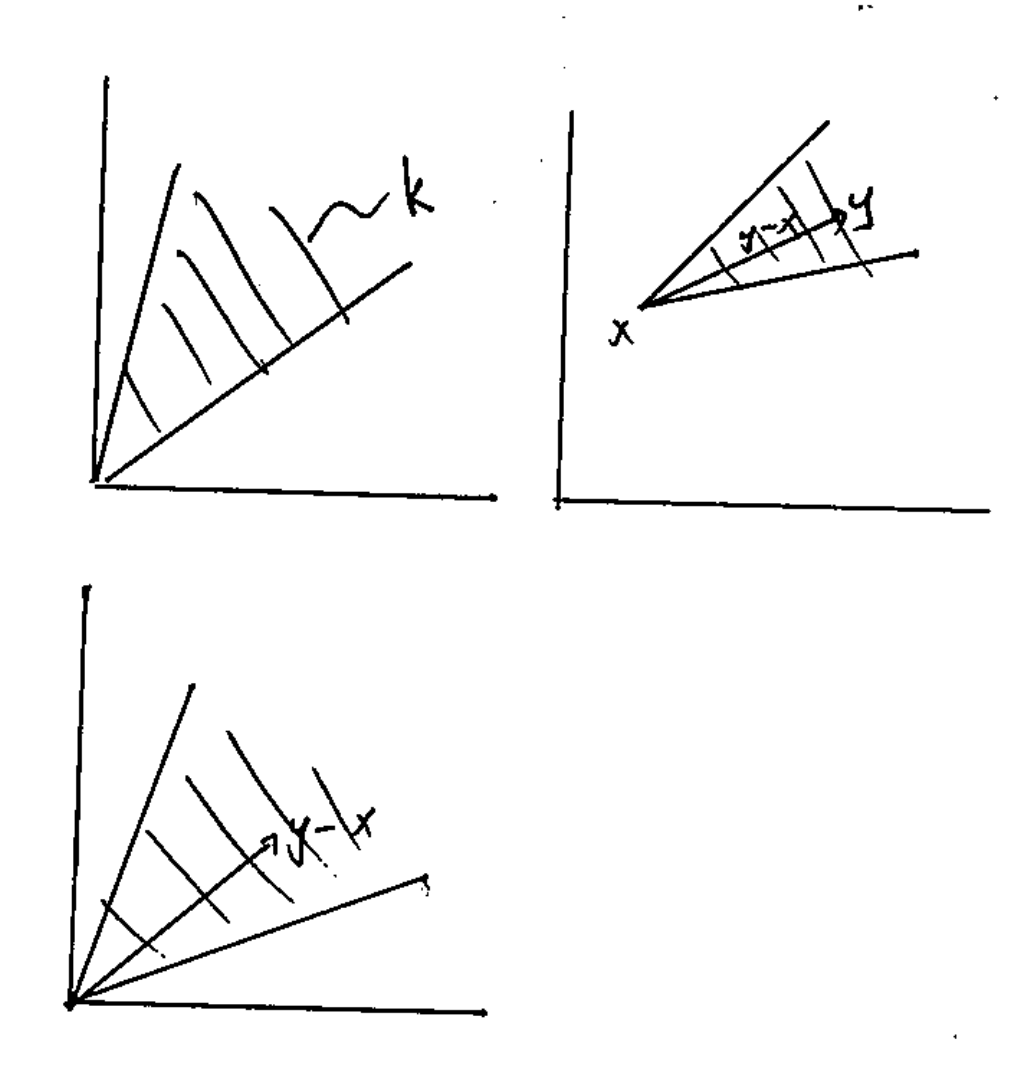
\includegraphics[width=1.8in,height=1.8in]{figures/ch08/figure1030_1.png}
	%\caption{This is an inserted JPG graphic} 
	%\label{fig:graph} 
\end{marginfigure}


\begin{example}
	$k = S^n_+$ ordering of matrices, elements of vector space are in $S^n$
	
	$X\leq_k y$ means $y-x\in S^n_+	$
	
	$\rightarrow$ is it true that $v^T(y-x)x \geq 0$, $\forall v$
	
	$\rightarrow$ are all eigenvalues non-negative
	
	Note: Interior of $S_+^n$ is $S^n_{++}$
	
	$x\leq_{S^n_+}y$
\end{example}

The 2 generalized inequalities come up so often, they are default.

\begin{enumerate}
	\item If compare 2 vectors $x,y\in \Re^n$, write $x\leq  y\Leftrightarrow x\leq_{\Re^n_{+}}y \Leftrightarrow y-x\in \Re^n_{+}$ 
	
	\item If compare 2 symmetric matrices, write:
	
	\begin{align*}
	x\leq y &\Leftrightarrow x\leq_{S_+^n} y\Leftrightarrow y - x\in S^n_{++}\\
	x< y &\Leftrightarrow y - x\in S^n_{+}
	\end{align*}
\end{enumerate}

\begin{example}
	$\{x\in \Re^n | x_1A_1 + x_2A_2 + ... + x_nA_n \leq B\}$
\end{example}

where $A_i\in S^m$ $B\in S^m$

"linear matrix inequality"

$F(x) = B - \sum^n_{i=1}x_iA_i$ $\leftarrow$affine function of $x$

\begin{align*}
\{x\in \Re^n | x_1A_1 + x_2A_2 + ... + x_nA_n \leq B\}
 &= \{x\in \Re^n | F(x)\geq 0\}\\
 &= \{x\in \Re^n | F(x)\in S^n_+ \}\\
 &=F^{-1}(S^n_+)
\end{align*}
So, a convex set.\\


Properties of Convex Sets:


\begin{marginfigure}
	\centering
	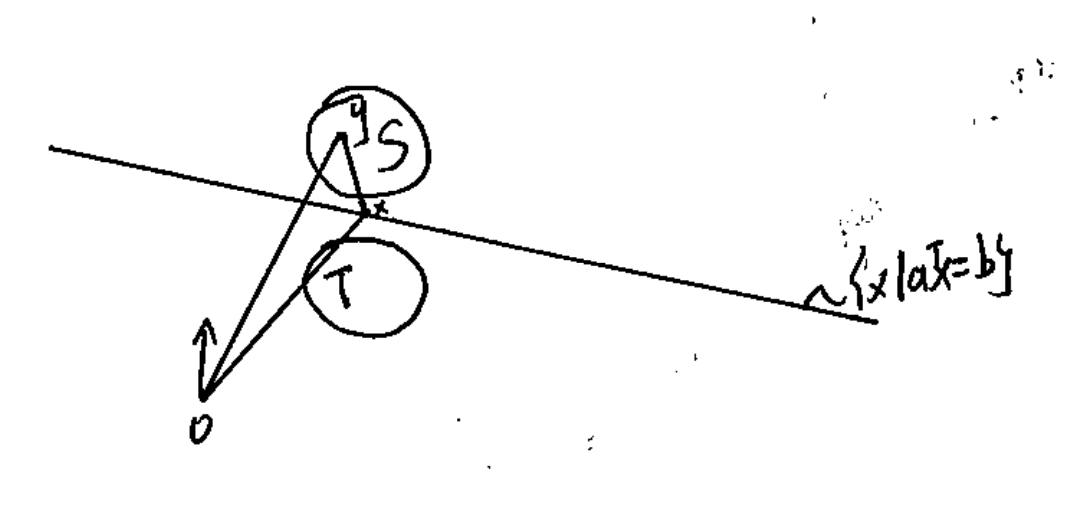
\includegraphics[width=1.8in,height=1.8in]{figures/ch08/figure1030_2.png}
	%\caption{This is an inserted JPG graphic} 
	%\label{fig:graph} 
\end{marginfigure}


\begin{enumerate}
	\item Separating hyperplane: If $S,T$ are convex sets in $\Re^n$ and disjoint, i.e, $S\cap T = \emptyset$, then there exists an $a \in \Re^n$ and $a,b\in \Re$ s.t.
	
	\begin{align*}
	a^Tx&\geq b, \forall x\in S\\
	a^Tx &<b, \forall x\in T
	a^Ty - a^Tx &= a^T(y-x) \geq 0
	\end{align*}
	
	\item Supporting hyperplanes:
	
	If $S$ is a convex set then $\forall x_0\in \delta \mathcal{S}$(boundary of $S$), $\exists a\in \Re^n$ s.t. 
	\begin{align*}
	a^Tx \leq a^Tx_0\\
	a^T(x - x_0)\leq 0
	\end{align*}
	
	\begin{marginfigure}
	\centering
	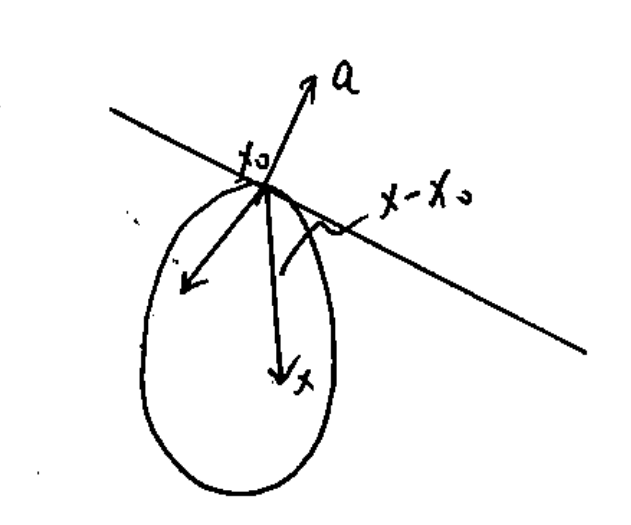
\includegraphics[width=1.8in,height=1.8in]{figures/ch08/figure1030_3.png}
	%\caption{This is an inserted JPG graphic} 
	%\label{fig:graph} 
	\end{marginfigure}
	
	\begin{marginfigure}
	\centering
	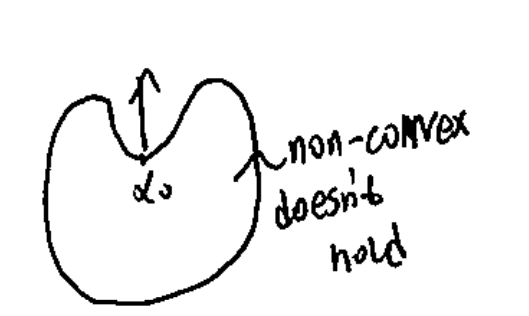
\includegraphics[width=1.8in,height=1.8in]{figures/ch08/figure1030_4.png}
	%\caption{This is an inserted JPG graphic} 
	%\label{fig:graph} 
	\end{marginfigure}
	
	\begin{marginfigure}
	\centering
	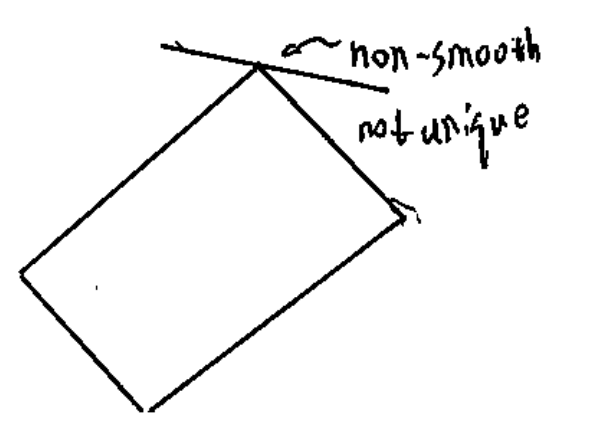
\includegraphics[width=1.8in,height=1.8in]{figures/ch08/figure1030_5.png}
	%\caption{This is an inserted JPG graphic} 
	%\label{fig:graph} 
	\end{marginfigure}
\end{enumerate}

\subsection{Convex Functions}
Let $F$ have aconvex domain, then $F:\Re^n\rightarrow \Re$ a convex function if $\forall x,y \in dom(F)$:

\begin{equation*}
F(\lambda x + (1-\lambda)y) \leq \lambda F(x) + (1-\lambda)F(y), \forall \lambda \in [0,1]
\end{equation*}

and strictly convex if 
\begin{equation*}
F(\lambda x + (1-\lambda)y) < \lambda F(x) + (1-\lambda)F(y), \forall \lambda \in (0,1)
\end{equation*}
.
Note: $F$ is a "concave" if $-F$ is convex.

\begin{marginfigure}
	\centering
	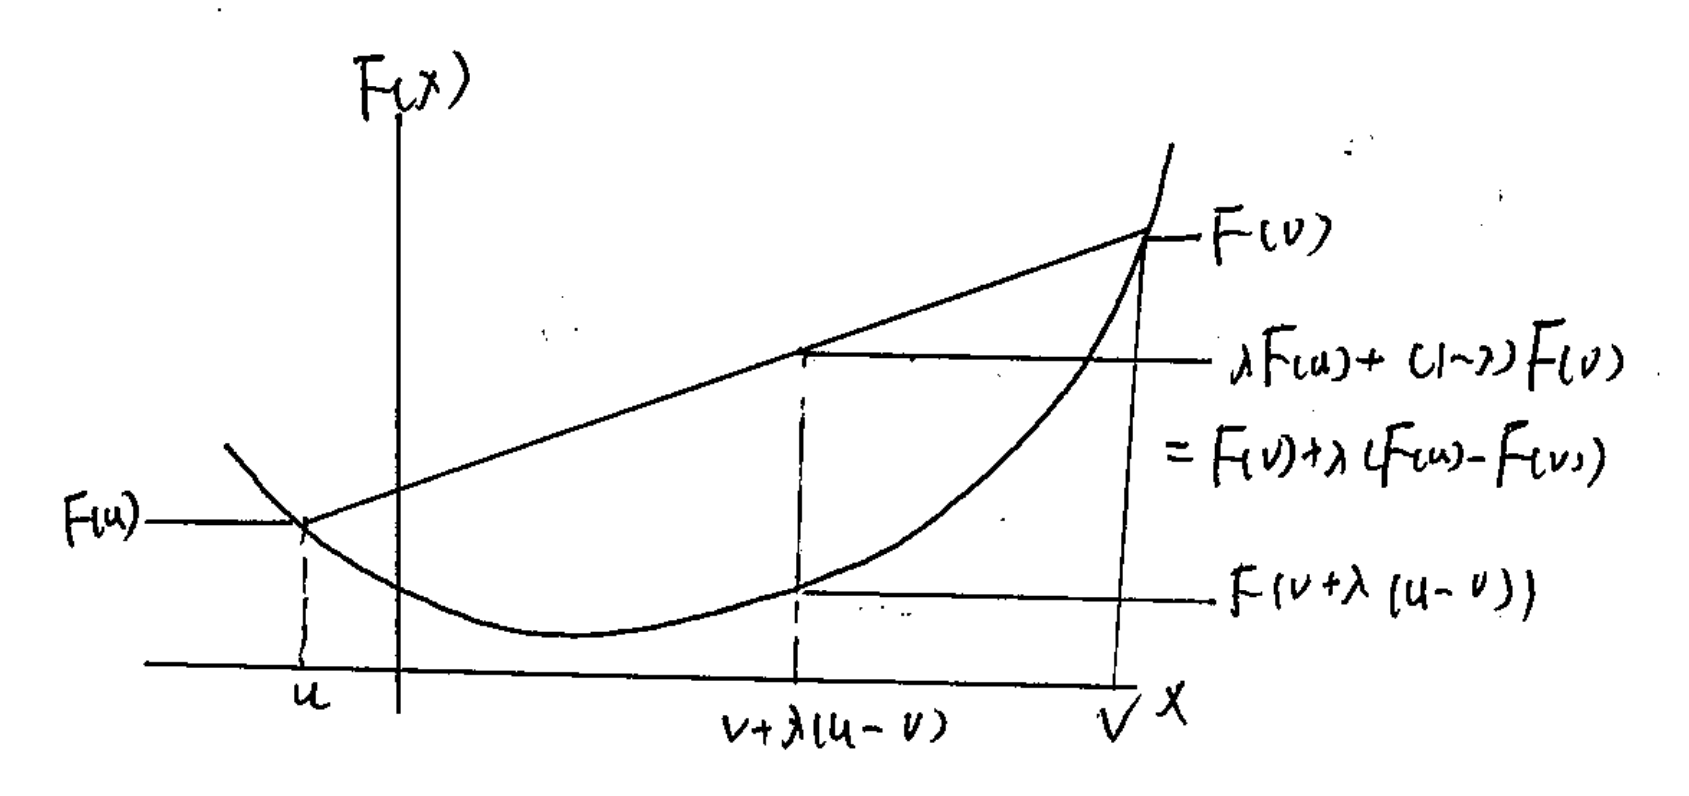
\includegraphics[width=1.8in,height=1.8in]{figures/ch08/figure1030_6.png}
	%\caption{This is an inserted JPG graphic} 
	%\label{fig:graph} 
\end{marginfigure}

Definition of convex:

\begin{equation*}
F(\lambda u + (1-\lambda)v) \leq \lambda F(u) + (1-\lambda)F(v)
\end{equation*}

And $F(\lambda u + (1-\lambda)v)$ can be written as $F(v + \lambda(u-v))$:

\begin{equation*}
F(\lambda u + (1-\lambda)v) \leq \lambda F(v) + \lambda(F(u)-F(v))
\end{equation*}

line segment connecting $(u,F(u))$ to $(v, F(v))$ always above buttom of bawl.


Sometimes define an "extended value" function

$$ \tilde{F}(x)=\left\{
\begin{array}{rcl}
F(x)       &      & \text{if } x\in dom(F)\\
\infty   &      & else
\end{array} \right. 
$$

Give an example:
\begin{itemize}
	\item Linear and affine
	
	\begin{marginfigure}
	\centering
	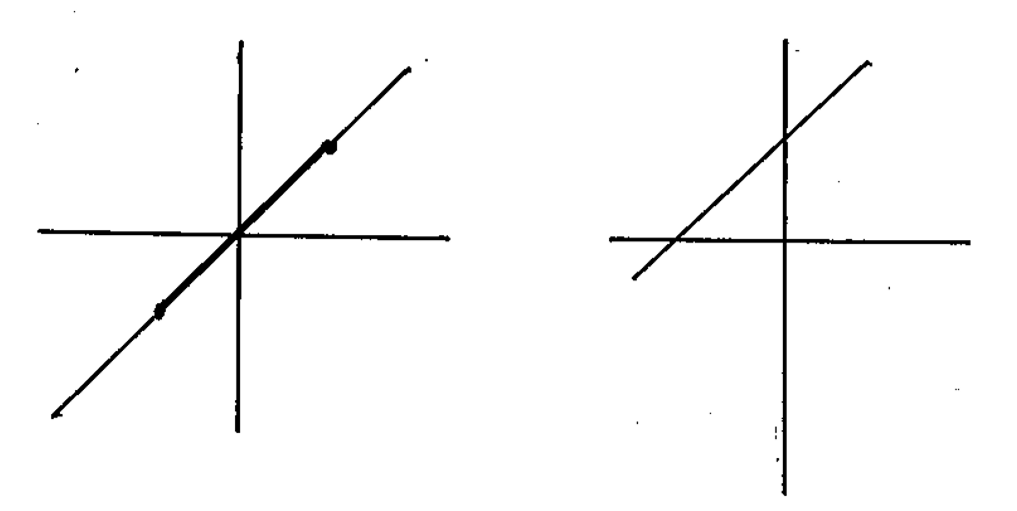
\includegraphics[width=1.8in,height=1.8in]{figures/ch08/figure1030_7.png}
	%\caption{This is an inserted JPG graphic} 
	%\label{fig:graph} 
	\end{marginfigure}
	
	both convex \& concave
	
	\item $x^2$ convex
	
	\begin{marginfigure}
	\centering
	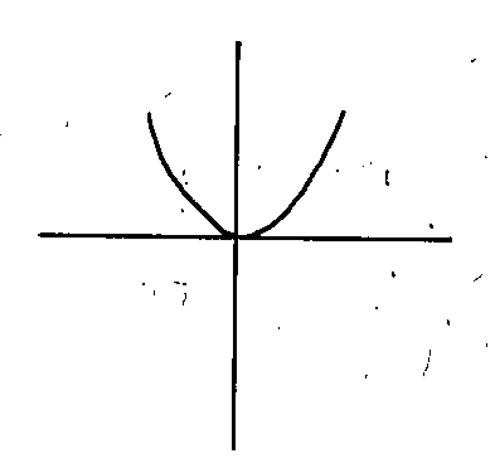
\includegraphics[width=1.8in,height=1.8in]{figures/ch08/figure1030_8.png}
	%\caption{This is an inserted JPG graphic} 
	%\label{fig:graph} 
	\end{marginfigure}
	
	\item $F(x) = logx$ with $domF = \Re_{++}$, concave
	
	\begin{marginfigure}
	\centering
	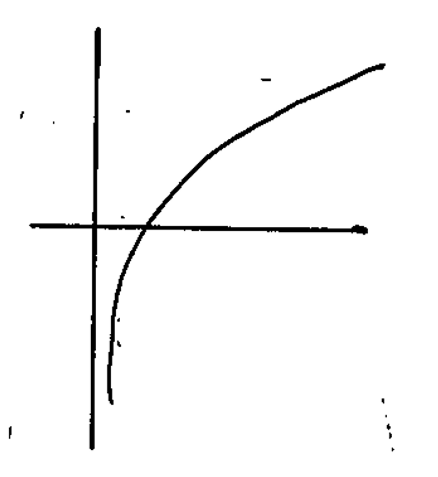
\includegraphics[width=1.8in,height=1.8in]{figures/ch08/figure1030_9.png}
	%\caption{This is an inserted JPG graphic} 
	%\label{fig:graph} 
	\end{marginfigure}
	
	\item $\Vert x\Vert$ is convex:
	
	\begin{align*}
	\Vert \lambda x + (1-\lambda)y\Vert &\leq \Vert \lambda x\Vert + \Vert(1-\lambda)y\Vert\\
	&= \lambda \Vert x \Vert + (1-\lambda)\Vert y \Vert
	\end{align*}
	
	\item $\frac{1}{x}$ convex on $\Re_{++}$, concave on $\Re_{--}$
	
	\begin{marginfigure}
	\centering
	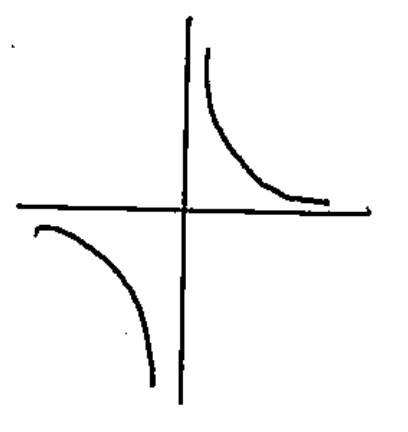
\includegraphics[width=1.8in,height=1.8in]{figures/ch08/figure1030_10.png}
	%\caption{This is an inserted JPG graphic} 
	%\label{fig:graph} 
	\end{marginfigure}
\end{itemize}

Recall: Epigraph of a function

\begin{equation*}
epiF = \{(x,t)|t\geq F(x), x\in domF \}
\end{equation*}

\begin{marginfigure}
	\centering
	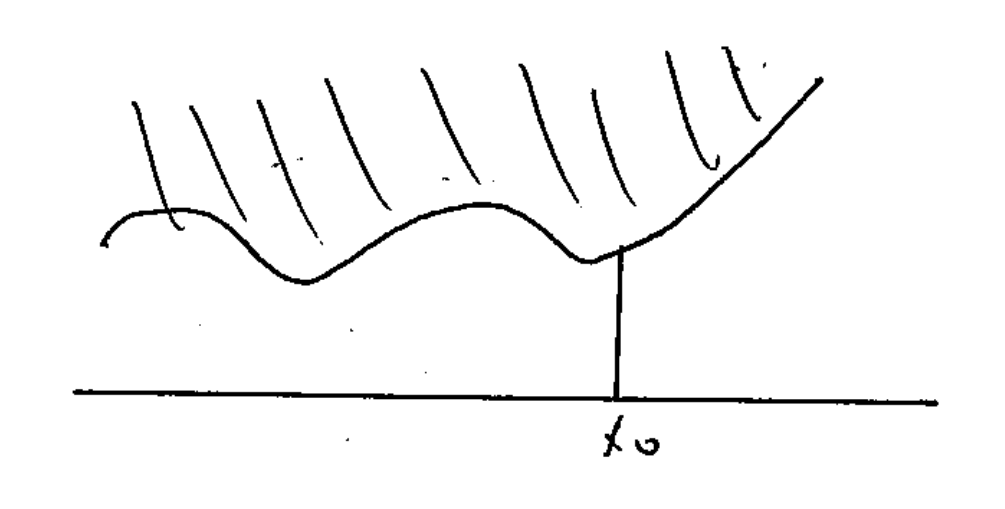
\includegraphics[width=1.8in,height=1.8in]{figures/ch08/figure1030_11.png}
	%\caption{This is an inserted JPG graphic} 
	%\label{fig:graph} 
\end{marginfigure}

\begin{definition}
	$f$ is a convex function iff $epif$ is a convex set
\end{definition}

\begin{definition}{Sublevel sets}
	$\mathcal{C}(\alpha) = \{x|F(x)\leq \alpha, x\in domF \}$.
	
	\begin{marginfigure}
	\centering
	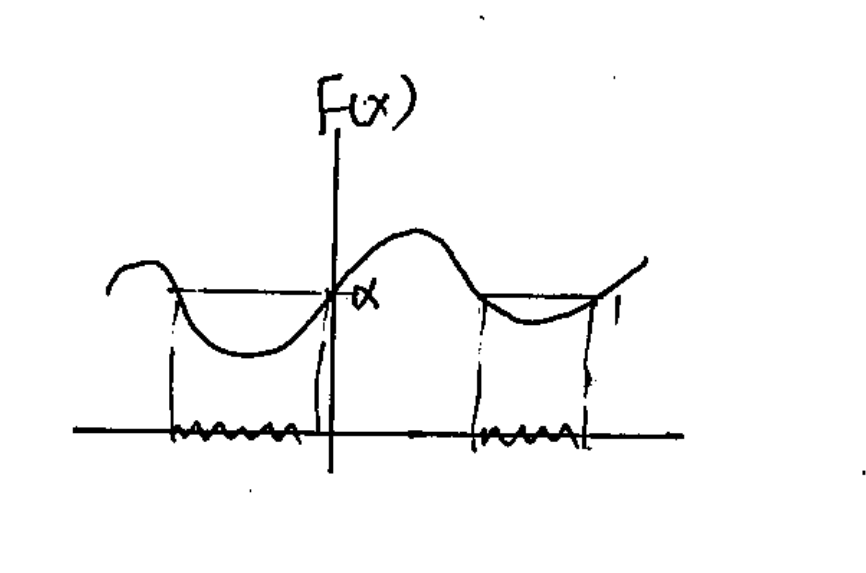
\includegraphics[width=1.8in,height=1.8in]{figures/ch08/figure1030_12.png}
	%\caption{This is an inserted JPG graphic} 
	%\label{fig:graph} 
	\end{marginfigure}
\end{definition}

\begin{theorem}
	If $F$ is convex, its sub-level sets are all convex sets.
\end{theorem}

Converse is nor true $\rightarrow$ if all sub-level sets of a function are convex sets, the function is "quasi-convex" but not necessarily convex.\\

\begin{marginfigure}
	\centering
	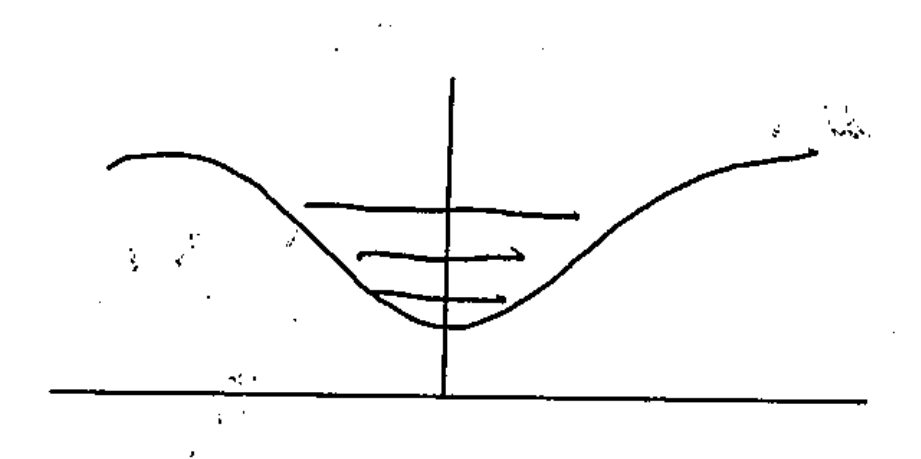
\includegraphics[width=1.8in,height=1.8in]{figures/ch08/figure1030_13.png}
	%\caption{This is an inserted JPG graphic} 
	%\label{fig:graph} 
\end{marginfigure}

1) Non-negative sums of convex functions are convex.

Let $F(x) =\sum^m_{i=1}a_iF_i(x)$, $domF = \cap^m_{i=1}domF_i$. 

\begin{align*}
F(\lambda x + (1-\lambda)y) &= \sum^m_{i=1}a_iF_i(\lambda x + (1-\lambda)y)\\
&\leq \sum^m_{i=1}a_i[\lambda F_i(x) + (1-\lambda)F_i(y)]\\
&= \lambda[\sum^m_{i=1}a_iF_i(\lambda)] + (1-\lambda)[\sum^m_{i=1}a_iF_i(y)]
\end{align*}

2) Convex functions of affine transformations of variables

Let $g(x) =F(Ax + b)$ where $F(\cdot)$ is convex.

\begin{align*}
g(\lambda x + (1-\lambda)y) &= F(A(\lambda x + (1-\lambda)y) + b)\\
&= F(\lambda(Ax + b) + (1-\lambda)F(Ay+b))\\
&\leq \lambda F(Ax + b) + (1-\lambda)F(Ay+b)\\
&= \lambda g(\lambda) + (1-\lambda)g(y)
\end{align*}

\begin{equation*}
dom(g) = \{x|Ax + b \in domF \}
\end{equation*}


3) The max of a pair of convex functions is a convex function:

\begin{equation*}
g(x) = max\{F_1(x), F_2(x) \}
\end{equation*}


\begin{marginfigure}
	\centering
	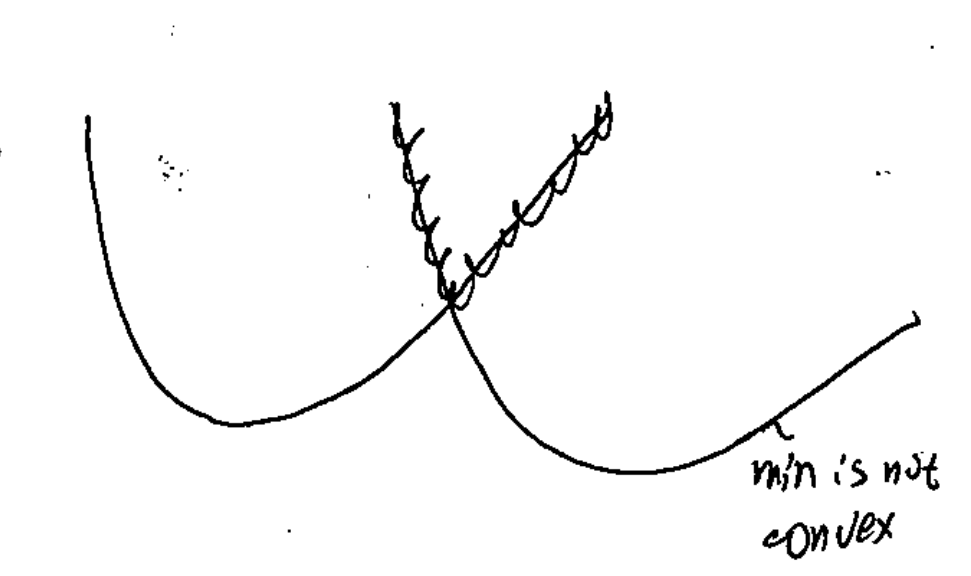
\includegraphics[width=1.8in,height=1.8in]{figures/ch08/figure1030_14.png}
	%\caption{This is an inserted JPG graphic} 
	%\label{fig:graph} 
\end{marginfigure}
%Above are notes for Oct30

%Below are notes for Nov 4
\subsection{Cones and generalized inequalities}

\begin{align*}
F(x) &=\sum\alpha_iF_i(x)\\
g(x) &= F(Ax + b)\\
g(x) &= max\{F_1(x), F_2(x) \}
\end{align*}

Example 1:
\begin{align*}
F(x) &= \sum^{\infty}_{i=1}log(b_i - a_i^Tx)^{-1}\\
&=\sum^n_{i=1}-log(b_i - a_i^Tx)
\end{align*}
where $\lambda \in \Re^n$, $a_i\in \Re^n$, $b_i\in \Re$

1) Note: $-log(\cdot)$ is a convex function, $dom\, -log(\cdot) = R_{++}$, $domF = \{x|b_i - a_i^Tx >0, \forall i\in [m] \} =\{x|b_i - a_i^Tx \in \Re_{++}, \forall i\in [m]$. Inverse image of $\Re_{++}$ under an affine transformation, and therefore a convex set. 

2) Sum of convex functions each a convex function of an affine transformation of $x$, $\Leftrightarrow$ Therefore a convex function.\\

\begin{example}
	
\begin{marginfigure}
	\centering
	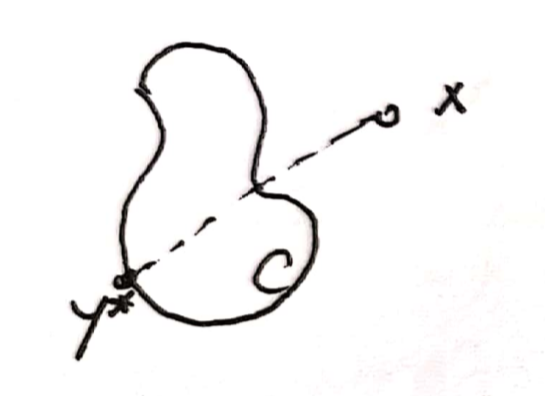
\includegraphics[width=1.8in,height=1.8in]{figures/ch08/figure1104_1.png}
	%\caption{This is an inserted JPG graphic} 
	%\label{fig:graph} 
\end{marginfigure}

\begin{equation*}
F(x) = sup_{y\in \mathcal{C}}\Vert y-x\Vert
\end{equation*}

note $\mathcal{C}$ not necessarily a convex set. 

\begin{enumerate}
	\item $y-x\rightarrow$ affine and therefore convex function of $x$.
	
	\item $\Vert\cdot\Vert\rightarrow$ norm function, so a convex function of its argument. 
	
	\item F(x) = $sup_{y\in \mathcal{C}}\Vert y-x\Vert$, $y\in \mathcal{C}$ is the basic max of a bunch of convex functions, each indexed by a $y\in \mathcal{C}$
\end{enumerate}
\end{example}

\begin{example}
	


\begin{equation*}
F(x) =inf_{y\in \mathcal{C}}\Vert y-x\Vert
\end{equation*}

$\rightarrow$ generally NOT convex in $x$.

$\rightarrow$ If $\mathcal{C}$ is a convex set, then this is convex in $x$. 
\end{example}

\subsection{Projection} If $h(x, y)$ is convex in $(x,y)$, then $F(x) = inf_yh(x,y)$ is convex in $x$.

\begin{marginfigure}
	\centering
	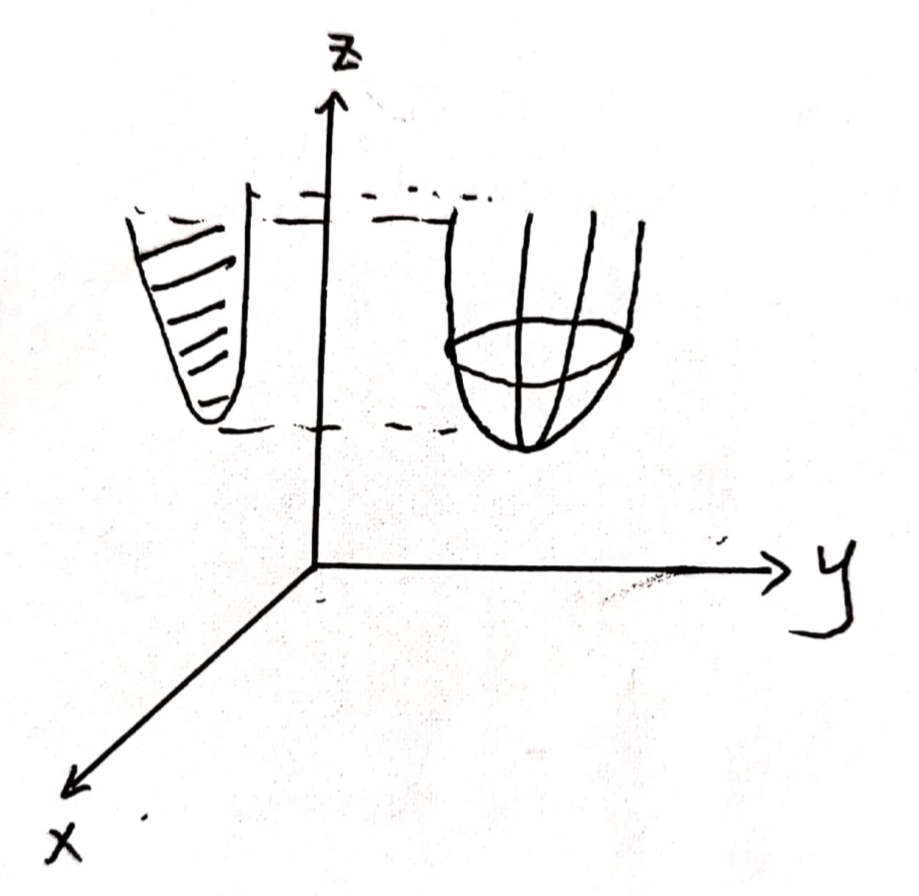
\includegraphics[width=1.8in,height=1.8in]{figures/ch08/figure1104_2.png}
	%\caption{This is an inserted JPG graphic} 
	%\label{fig:graph} 
\end{marginfigure}

Idea: Shine light along $y$-axis, get shadow on $x-z$ plane that shadow is epif \& is a convex set. 

\begin{proof}
	Since $h(x,y)$ is convex in $\begin{bmatrix}
	x\\
	y
	\end{bmatrix}\in domh$,
	\begin{equation*}
	epih = \{(x,y,t)|t\geq h(x,y), \begin{bmatrix}
	x\\
	y
	\end{bmatrix}\in domh \}
	\end{equation*}
	$\rightarrow$ That's the black bowl in above graph. 
	
	Now consider:
	\begin{equation*}
	F(x) = inf_{y:\begin{bmatrix}
		x\\
		y
		\end{bmatrix}\in domh}h(x,y)
	\end{equation*}
	
	\begin{align*}
	domF &= \{x|\exists y s.t. (x,y)\in domh \}\\
	&= \{\begin{bmatrix}
	1&0
	\end{bmatrix}\begin{bmatrix}
	x\\
	y
	\end{bmatrix} \vert \begin{bmatrix}
	x\\
	y
	\end{bmatrix}\in domh \}
	\end{align*}
	
	Above: affine map of all points in a convex set and therefore domf is a convex set.
\end{proof}

\begin{align*}
epiF &= \{(x,t)|t\geq inf_{y:\begin{bmatrix}
	x\\
	y
	\end{bmatrix}}\in domh, x\in domf \}\\
&= \{\begin{bmatrix}
\cdots
\end{bmatrix}\begin{bmatrix}
x\\
y\\
t
\end{bmatrix}\vert t\geq h(x,y), \begin{bmatrix}
x\\
y
\end{bmatrix}\in domh \}
\end{align*}

So this set is a convex set. But this set if $epiF$ so $F$ must be a convex function. 

\begin{example}
	


\begin{equation*}
F(x) = inf_{y\in\mathcal{C}}\Vert x-y\Vert
\end{equation*}
is a convex function if $\mathcal{C}$ is a convex set. 

\begin{enumerate}
	\item $x-y$ is affine in $x$
	
	\item $\Vert\cdot\Vert$ is a convex function for all norms.
	
	\item Apply projection theorem where $domh = \{\begin{bmatrix}
	x\\
	y
	\end{bmatrix}\vert x\in \Re^n, y\in \mathcal{C} \}$ is a convex set and $x$ is unconstrained. 
\end{enumerate}
\end{example}
\subsection{Characterizing Convexity by Restricting to a Line}

Theorem: $F: \Re^n \rightarrow \Re$ is convex iff $g:\Re \rightarrow \Re$ is convex (in $t$) where $g(t) =F(x_0 + tv)$. For all choices of $x_0\in domf$, $v\in \Re^n$, $t\in \Re$ s.t. $x_0+tv\in domF$

\begin{itemize}
	\item $g(t)$ is function restricted to a line/slice
	
	\item If all possible slices convex then so is $F$.
\end{itemize}

Note: need $x_0+tv\in domF$, also note $domF$ is a convex set. 

\begin{equation*}
g(t) = g_{x_0, v}(t) = F(x_0+tv)
\end{equation*}

\begin{equation*}
dom(g_{x_0, v}) = \{t|x_0+tv \in domF \}
\end{equation*}

Therefore $dom(g_{x_0, v})$ is convex set for all $x_0, v$.\\

First, If $F$ is convex $\rightarrow$ $g$ convex. 
\begin{align*}
\forall t_1, t_2\in domg, \lambda\in [0,1]\\
g(\lambda t_1 +(1-\lambda)t_2) &= F(x_0+[\lambda t_1+(1-\lambda)t_2]v)\\
&= F(\lambda[x_0 +t, v]+(1-\lambda)[x_0+t_2v])\\
&\leq \lambda F(x_0+t_1 v)+(1-\lambda)F(x_0+t_2v)\\
&=\lambda g(t_1) + (1-\lambda)g(t_2)
\end{align*}

Second, $g$ convex in $t$, $\forall(x_0, v)\Rightarrow$ $F$ is convex. Pick arbitrary $x,y\in domF$, let $x_0 =x$, $v=(y-x)$, consider $g_{x_0, v}(t)$ for $t\in[0,1]$:

\begin{align*}
g_{x_0, v}(t) &= F(x_0+tv)\\
&= F(x+t(y-x))\\
&= F((1-t)x+ty)
\end{align*}
Since $g_{x_0, v}$ is convex in $t$ $\Rightarrow$ $F$ is convex in $t$. ($t$ plays role of $\lambda$)

\begin{example}
	


\begin{equation*}
F(x) =logdet(x^{-1})
\end{equation*}

\begin{itemize}
	\item $domF = S^n_{++}$ $\leftarrow$ PD matrices
	
	\item $S^n_{++} \subset S^n \leftarrow$ vector space of $n\times n$ symmetric matrices. 
\end{itemize}
To show this is a convex function, will show it is convex for all "lines".

line in $S^n$: $x_0 + tH$ where $x_0$ is synnetric PD matrix, $t\in \Re$ and $H$ is symmetric matrix in $S^n$. So $x_0 + tH$ is a family of symmetric matrices.

\begin{marginfigure}
	\centering
	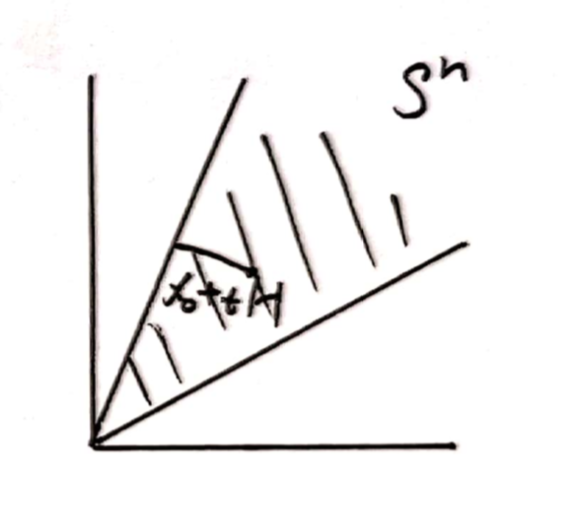
\includegraphics[width=1.8in,height=1.8in]{figures/ch08/figure1104_3.png}
	%\caption{This is an inserted JPG graphic} 
	%\label{fig:graph} 
\end{marginfigure}
\end{example}

note: $x_0\in S^n_{++}$, so $x_0^{-1}$exists, so $x_0^{\frac{1}{2}}$exists. $det(AB) = det(A)\cdot det(B)$

\begin{align*}
g(x) &= logdet(x_0+tH)^{-1}\\
&= logdet[(x_0^{\frac{1}{2}}x_0^{\frac{1}{2}}+tx_0^{\frac{1}{2}}x_0^{-\frac{1}{2}}+Hx_0^{-\frac{1}{2}}x_0^{\frac{1}{2}})^{-1}]\\
&= logdet[x_0^{-\frac{1}{2}}(I+tx_0^{-\frac{1}{2}}Hx_0^{-\frac{1}{2}})^{-1}x_0^{-\frac{1}{2}}]\\
&= logdetx_0^{-1} + logdet[(I+tx_0^{-\frac{1}{2}}Hx_0^{-\frac{1}{2}})^{-1}]\\
&= logdetx_0^{-1}+log(det(I+tM)^{-1})\\
&= logdetx_0^{-1}+log[\prod^n_{i=1}(1+t\lambda_i)^{-1}]\\
&= logdetx_0^{-1} - \sum_{i=1}^nlog(1+t\lambda_i)
\end{align*}

Recall $det$ is product of eigenvalues. 

\begin{equation*}
(I+tM)v = v+t\lambda v = (1+t\lambda)v
\end{equation*}
eigenvalues of $(I+tM)$ are $1+t\lambda_i$.\\

Note:

\begin{enumerate}
	\item $1+t\lambda_i$ is affine in $t$
	
	\item $-log(\cdot)$ convex
	
	\item sum of convex functions $\Rightarrow$ $g(t)$ is convex in $t$.
\end{enumerate}


%Above are notes for Nov 4




%Below are notes for Nov 6

$F(x) = \lambda_{max}(x)$ where $domF = S^n$ is convex. 

(a) 

\begin{align*}
\lambda_{max}(x) &= max_{v:\Vert v\Vert = 1}v^TXv\\
v^TXv &= v^TQ\Lambda Q^Tv = \tilde{v}^T\Lambda \tilde{v}\\
&= \sum^n_{i=1}(\tilde{v}_i)^2\lambda_i \leq \lambda_{max}(X)
\end{align*}

(b)
\begin{equation*}
v^T(\alpha x_1 + \beta x_2)v = \alpha v^Tx_1v + \beta v^Tx_2v
\end{equation*}


$v^TXv$ is linear in $X$.

So $F(x)$ is $max$ of a bunch of functions linear in $X$ $\Leftarrow$ convex.

\begin{enumerate}
	\item $F(x) = \sigma_1(x)$ convex on $domF =\Re^{n\times m}$.
	
	\item $F(x) = (detX)^{\frac{1}{n}}$ , concave on $domf = S^n_{++}$
\end{enumerate}


\subsection{"First-order" condition}

\begin{theorem}
	A differentiable function $f$ ($domf$ is open and gradients exist everywhere in domain) is convex if and only if $\forall x,y\in domf$:
	\begin{equation*}
	F(y)\geq F(x) + \triangledown F(x)^T(y-x) \,\,\,\,\,  (*)
	\end{equation*}
	and if strictly convex if $(*)$ is a strict inequality for all $x\neq y$.
	
	\begin{marginfigure}
	\centering
	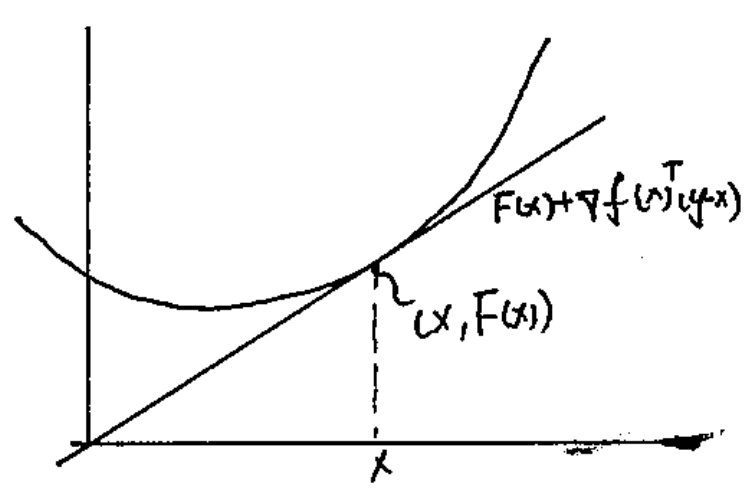
\includegraphics[width=1.8in,height=1.8in]{figures/ch08/figure1106_1.png}
	%\caption{This is an inserted JPG graphic} 
	%\label{fig:graph} 
	\end{marginfigure}
	
	$\rightarrow$ First-order Taylor approximation is everywhere an under-estimator of $f$.
	
	$\rightarrow$ There is a tangent plane that is a supporting hyperplane of $epiF$.
\end{theorem}

First, assume $f$ convex $\Rightarrow$ show $(*)$ holds. Pick $(x,y)$ by define convex function. 

\begin{align*}
F((1-\lambda)x+\lambda y) &\leq (1-\lambda)F(x) + \lambda F(y)\\
\frac{F(x+\lambda(y-x)) - F(x)}{\lambda} &\leq F(y) - F(x)
\end{align*}


Let $\lambda \rightarrow 0$ and observe $lim_{\lambda\rightarrow 0} \frac{F(x+\lambda(y-x)) - F(x)}{\lambda} = \triangledown F(x)^T(y-x)$.

\begin{equation*}
\triangledown F(x)^T(y-x)\leq F(y) - F(x)
\end{equation*}

(You can also do above procedure in 1-dimension, try it by yourself)

Secondly, assume $(*)$ holds $\rightarrow$ show convex.

Take any $(x,y)\in domf$, then $\forall \lambda\in[0,1]$, $z= \lambda x + (1-\lambda)y \in domf$ since $domf$ convex.

Using $(*)$ 2 times get:

\begin{align*}
F(x) &\geq F(z) + \triangledown F(x)^T(x-z)\\
F(y) &\geq F(z) + \triangledown F(x)^T(y-z)
\end{align*} 
Compute

\begin{align*}
\lambda F(x)+(1-\lambda)F(y) &\geq F(z) + \triangledown F(z)^T[\lambda (x-z)+(1-\lambda)(y-z)]\\
&= F(z) + \triangledown F(z)^T[\lambda x - \lambda z + y - z - \lambda y +\lambda z]\\
&= F(z) + \triangledown F(z)^T[\lambda x + (1-\lambda)y - z]\\
&= F(z)\\
&= F(\lambda x + (1-\lambda )y)
\end{align*}

Connect $1^{st}-$order condition with $epif$

Recall $(x,t)\in epif$ if $t\geq F(x)$

$1^{st}-$order condition: $\forall x,y \in domf$, $F(y)\geq F(x) + \triangledown F(x)^T(y-x)$

\begin{marginfigure}
	\centering
	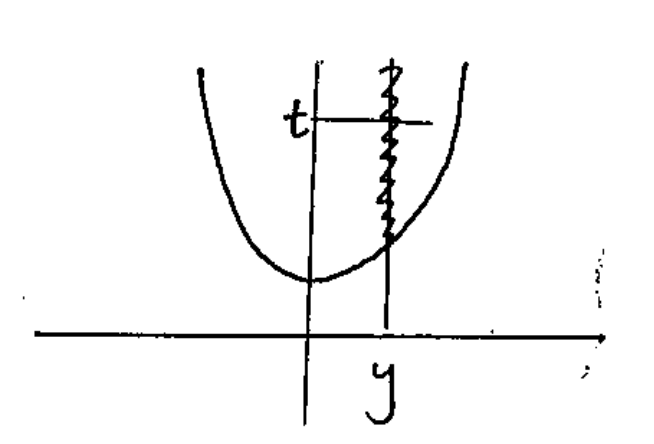
\includegraphics[width=1.8in,height=1.8in]{figures/ch08/figure1106_2.png}
	%\caption{This is an inserted JPG graphic} 
	%\label{fig:graph} 
\end{marginfigure}

Consider and $(y,t)\in epif$:

\begin{align*}
t &\geq F(y) \geq F(x) + \triangledown F(x)^T(y-x)\\
0 &\geq F(x) - t + \triangledown F(x)^T(y-x)\\
&= \begin{bmatrix}
\triangledown F(x)^T & -1
\end{bmatrix}\begin{bmatrix}
y-x\\
t -F(x)
\end{bmatrix}\\
&= \begin{bmatrix}
\triangledown F(x)^T  & -1
\end{bmatrix}\begin{bmatrix}
y\\
t
\end{bmatrix} + (-\triangledown F(x)^Tx + F(x))
\end{align*}

\begin{marginfigure}
	\centering
	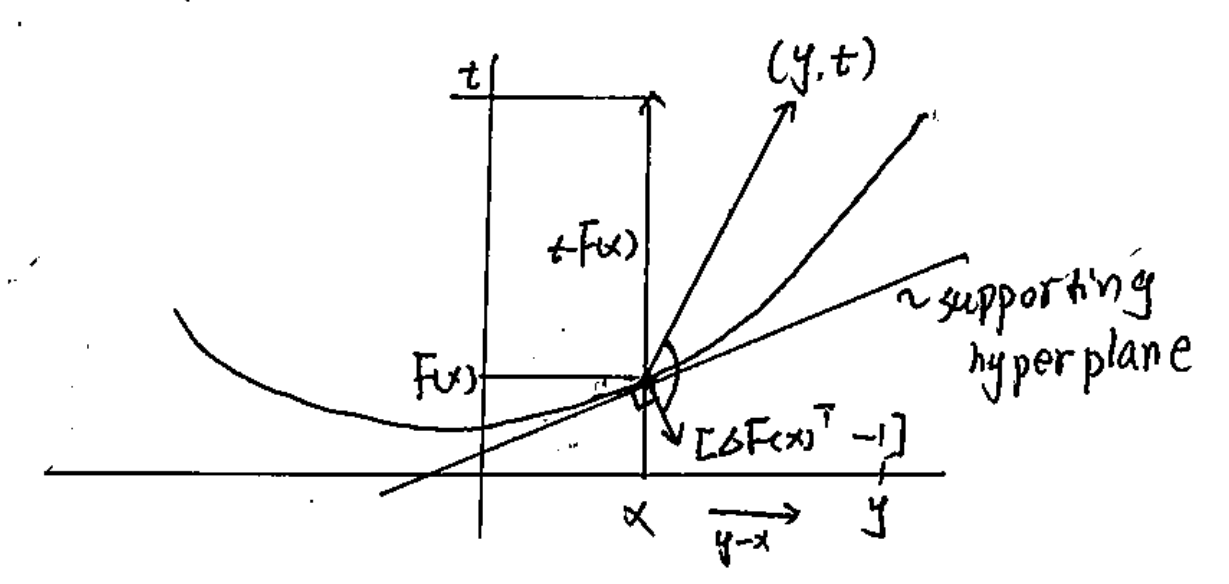
\includegraphics[width=1.8in,height=1.8in]{figures/ch08/figure1106_3.png}
	%\caption{This is an inserted JPG graphic} 
	%\label{fig:graph} 
\end{marginfigure}

\subsection{"Second-order" condition}

\begin{theorem}
	If $f$ is everywhere twice differentiable, then $f$ is convex if and only if its Hessian $\triangledown^2F(x)\geq 0$(PSD) for all $x\in domf$
\end{theorem}

Similarly, we show our two-parts proof:\\

Firstly, assume $f$ convex $\Rightarrow$ show $\triangledown^2F(x)\geq 0$.

Let $x_o \in domf$(any point), $v\in \Re^n$(a direction), then $z = x_0 + \lambda v$ is in $domf$ if $\lambda > 0$ sufficiently small. 

By Taylor approximation, 
\begin{equation*}
F(z) = F(x_0) + \triangledown F(x_))^T(\lambda v) + \frac{1}{2}(\lambda_v)^T\triangledown^2F(x_0)\lambda v + O(\lambda^3)
\end{equation*}

Re-arrange:

\begin{equation*}
\frac{1}{2}\lambda^2v^T\triangledown^2F(x_0)v+O(\lambda^3) =       F(z) - F(x_0) - \triangledown F(x_0)^T(\lambda v)
\end{equation*}

The right-hand side is $\geq 0$ by first-order-convexity result.\\ 





Continuing, divide through by $\lambda^2$ to get:
\begin{equation*}
\frac{1}{2}v^T\triangledown^2F(x_0)v + \frac{O(\lambda^3)}{\lambda^2} \geq 0
\end{equation*}

In above equation, $O(\lambda^3)$ means this is $\leq M\lambda^3$ "Big-O", so $\frac{O(\lambda^3)}{\lambda^2} \leq M\lambda$.

Letting $\lambda\rightarrow 0$ get $\frac{1}{2}v^T\triangledown^2F(x_0)v\geq 0$, $\Rightarrow \triangledown^2F(x_0)$ is PSD. 

For all $x_0 \in domf$, since $v\in \Re^n$ can be chosen arbitrarily. \\

Secondly, Assume $\triangledown^2F(x_0)\geq 0, \forall x_0\in domf$ $\Rightarrow$ convex.

Apply Taylor approximation with remainder $\forall x,y\in domf$, 

\begin{equation*}
F(y) =F(x) + \triangledown F(x)^T(y-x) + \frac{1}{2}(y-x)^T\triangledown^2F(z)(y-x)
\end{equation*}

where Hessian evaluated at some $z$ between $x\& y$("mean value")

Since $\triangledown^2F(x_0)\geq 0$,

\begin{equation*}
F(y) \geq F(x) + \triangledown F(x)^T (y-x)
\end{equation*}

$\rightarrow$ back to $1^{st}-$order-condition, true for $\forall x,y$. So $f$ must be convex. 


Here we can give some examples:

\begin{enumerate}
	\item $F(x) = x^2$, $domf = \Re$, $F''(x) = 2 > 0$, $\forall x\in \Re$(strictly convex)
	
	\item $F(x) = x^3$, $domf = \Re$, $F'(x) = 3x^2$, $F''(x) = 6x$, but if set $demf = \Re_+$ then $f$ is convex.
	
	\item $F(x) = x^{\alpha}$, $domf = \Re_+$, $F''(x) = \alpha(\alpha - 1)x^{\alpha - 2}$ where $\alpha(\alpha - 1) > 0$ if $\alpha > 1$ or $\alpha < 0$ and $\alpha(\alpha - 1) < 0$ if $0<\alpha < 1$. $x^{\alpha - 2}\geq 0$ since $domf = \Re_+$
	
	\begin{marginfigure}
	\centering
	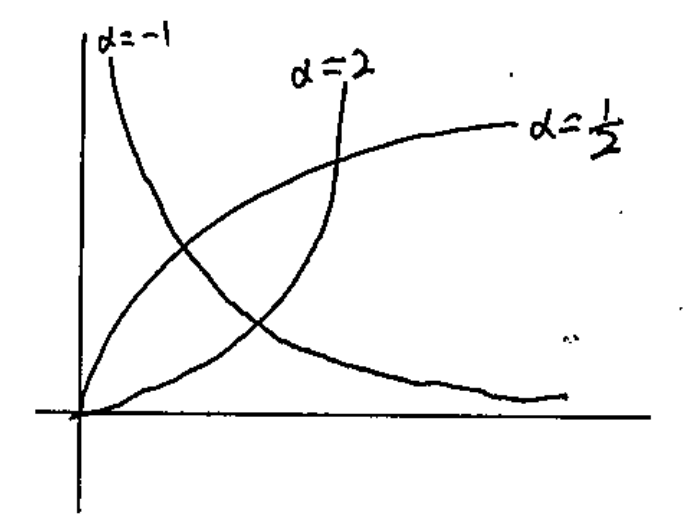
\includegraphics[width=1.8in,height=1.8in]{figures/ch08/figure1106_4.png}
	%\caption{This is an inserted JPG graphic} 
	%\label{fig:graph} 
	\end{marginfigure}
	
	\item $F(x) = log_ex$, $domf = \Re_{++}$, $F'(x) = \frac{1}{x}$, $F''(x) = -\frac{1}{x^2}<0$, concave.
	
	\item $F(x) = xlog_e(x)$, $domf = \Re_{++}$, $\frac{\alpha^2}{\alpha x^2}F(x) = \frac{\alpha}{\alpha x}[log_e(x) + \frac{x}{x}] = \frac{1}{x} > 0$, convex
	
	\item $F(x) = e^{\alpha x}$, $domf = \Re$, $F''(x) = \alpha^2 e^{\alpha x}$
	
	\item $F(x) = \frac{1}{2}x^THx + c^Tx + d$, 
	
	\begin{align*}
	\triangledown F(x) &= \frac{1}{2}(H+H^T)x + c \\
	&= \tilde{H}x + c\\
	\triangledown^2F(x) &= \tilde{H}
	\end{align*}
	If $\tilde{H}\geq 0$, then convex.
	
	If $\tilde{H}\leq 0$, then concave.
	
	If neither PSD or negative semi-definite, then neither. 
\end{enumerate}

\begin{example}
	\begin{align*}
	F(x,y) &= x^2 + y^2 + 3xy \\
	&= \begin{bmatrix}
	x&y
	\end{bmatrix}\begin{bmatrix}
	1&\frac{3}{2}\\
	\frac{3}{2} & 1
	\end{bmatrix}\begin{bmatrix}
	x\\
	y
	\end{bmatrix}\\
	&=\frac{1}{2}\begin{bmatrix}
	x&y
	\end{bmatrix}\begin{bmatrix}
	2&3\\
	3 & 2
	\end{bmatrix}\begin{bmatrix}
	x\\
	y
	\end{bmatrix}\\
	det(\begin{bmatrix}
	2&3\\
	3&2
	\end{bmatrix} - \lambda I) &= det\begin{bmatrix}
	2-\lambda & 3\\
	3 & 2-\lambda
	\end{bmatrix}\\
	&= (2-\lambda)^2 - 9\\
	&= (\lambda - 5)(\lambda + 1)
	\end{align*}
	Try $-45^{\circ}$ line, will see slice is not convex.
	
	\begin{equation*}
	F(x,-x) = x^2 + (-x)^2 + 3x(-x) = 2x^2 - 3x^2 = -x^2
	\end{equation*}
	
\end{example}

\begin{example}
	Geometric mean $\sqrt{x_1x_2} = F(x_1x_2)$, $domf = \Re_+ \times \Re_+$.
	
	\begin{equation*}
	\triangledown^2F(x) = -\frac{\sqrt{x_1x_2}}{y}\begin{bmatrix}
	\frac{1}{x^2_1} & -\frac{1}{x_1x_2}\\
	-\frac{1}{x_1x_2} & \frac{1}{x^2_2}
	\end{bmatrix}
	\end{equation*}
	
	1) Calculate eigenvalues
	
	2) Use definition
	
	\begin{align*}
	v^T\triangledown^2F(x)v &= -\frac{\sqrt{x_1x_2}}{2}[\frac{v_1^2}{x_1^2} - \frac{2v_1v_2}{x_1x_2} + \frac{v_2^2}{x^2_2}]\\
	&= -\frac{\sqrt{x_1x_2}}{2}(\frac{v_1}{x_1} -\frac{v_2}{x_2}) \leq 0
	\end{align*}
	
	Concave in $(x_1, x_2)$, $F(x) = (\prod^n_{i=1}x_i)^{\frac{1}{n}}$ is concave in $x\in \Re^n$
\end{example}

Consequence of convexity conditions for differentiable $f$

By $1^{st}-$order, if $f$ convex, then:

\begin{equation*}
F(y)\geq F(x) + \triangledown F(x)^T(y-x), \forall x,y\in domf
\end{equation*}


what if $\triangledown F(x^*) = 0 \in \Re^n$ for some $x^*\in domf$:
\begin{equation*}
F(y)\geq F(x^*) + \triangledown F(x^*)^T(y-x^*)
\end{equation*}

So if you can find an $x^*\in domf$ s.t. $\triangledown F(x^*) = 0$ then that is a global minimum.

%Above are notes for Nov 6
